% The tangent space T_p(M) to S^1 at a point p, with a tangent vector v.
% Source: book/tex/diffgeo/manifolds.tex (§ Tangent spaces and bundles).
\documentclass[border=2mm]{standalone}
\usepackage{tikz}\usetikzlibrary{arrows.meta}\usepackage{amssymb}
\begin{document}
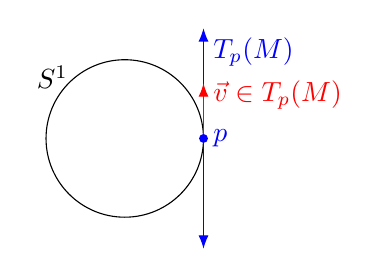
\begin{tikzpicture}
  \draw (0,0) circle (1); \node at (140:1.2){$S^1$};
  \draw[blue,{Latex}-{Latex}] (1,-1.4)--(1,1.4); \node[blue,below right] at (1,1.4){$T_p(M)$};
  \draw[red,-{Latex}] (1,0)--(1,0.7); \node[red,right] at (1,0.55){$\vec v\in T_p(M)$};
  \fill[blue] (1,0) circle (1.6pt) node[right,blue]{$p$};
\end{tikzpicture}
\end{document}
